\chapter{Background}
\label{chapter:background}

% 1. how the literature was collected (describe it pragmatically)
%
% 2. literature review (summary, analysis, and comparisons)
%
%   A literature review should answer:
%
%     * What do we already know about the topic?
%     * What do you have to say critically about what is already known?
%     * Has anyone else done anything exactly the same?
%     * Has anyone else done anything that is related?
%     * Where does your work fit in with what is done before?
%     * Why is your research worth doing in the light of what has
%       already been done?
%
%   A literature review should be a dialogic rather than a mere
%   replication of other peoples writing. Should not be a laundry
%   list of previous studies.
%
%   Be focused and critical. Include an incisive critique that will help your
%   peers see the world differently.
%
% 3. paragraph or two about my subject related to popular literature
%    (search Amazon or Library of Congress and say something like: there
%    were X books about this subject, the first was published in 2001
%    but the majority of books were published the last two years, and
%    maybe show a graph)

\section{Literature Search}
\label{section:literature.search}

Before the literature search was conducted we did some preliminary thinking
about
\begin{inparaenum}[(i)]
  \item the focus of our topic to get more precise results, and
  \item what literature databases would yield sufficient and accurate
    findings.
\end{inparaenum}
Based on these concerns we settled on the literature indexes laid out in
\tableref{literature.databases} and used the following keywords%
\sidenote{
  With varying use of modifiers (i.e. AND) or quotations to find exact phrases
}
for search:

\begin{items}
  \iterm{social navigation} is the concept of our main topic.
  \iterm{collaborative filtering} is often used to realize our
    main topic.
  \iterm{recommender system} can be an application of our main topic.
  \iterm{tagging} can be related to our topic depending on use.
\end{items}

\begin{table}
  \begin{tabular}{ll}

    Name & Type \\
    \midrule

    \abbr{ACM} Digital Library &
    Full-text \\

    The Collection of Computer Science Bibliographies &
    Bibliography \\

    Inspec Online &
    Reference \\

    \abbr{HCI} Bibliography &
    Bibliography \\

  \end{tabular}

  \caption{Literature Databases}
  \label{table:literature.databases}
\end{table}

In addition to keyword based search we also conducted citation searches on the
articles that in our opinion seemed to be the most important in the field.
The articles that we found relevant during our literature search phase was
collected and studied. During this process we eliminated articles by the same
authors where similar topics and implementations were discussed and focused on
either the most recent or the most representative article.

First we'll briefly discuss navigation and sociality both in general terms
and relating to the web. Then we'll concentrate on these two topics together
by looking at the research where social navigation is used
consciously as a concept. By this we mean the research where either social
navigation is defined, redefined or problems relating to the concept is
discussed with a basis in such definitions.
After our main survey of social navigation research we'll look at topics
which we believe can be included in the discussion of social navigation or are
closely related.

Some of the research that has been conducted in the space of
social navigation and related areas does not share our focus on the Web.
We still found much such research interesting in spite of their attention to
generalized problems or specific problems in other fields than the Web.

\section{Navigation}
Navigation was traditionally associated with controlling a vessel at sea to
a given destination.%
\sidenote{
  \emph{Navigate} is in fact derived from the two Latin words \emph{navis}
  meaning \val{ship} and \emph{agere} meaning \val{to drive}
  \citep[\p{756}]{anderson97}.
}
Since then it's been used to describe behavior related to safely finding ones
way whether one is driving a car, flying a plane or walking on foot. Maps
(a graphical representation of the medium one are navigating in)
and compass (a tool for connecting graphical maps to the physical world)
are often used as aids in this way finding.

When used in context of
computer systems navigation is essentially a metaphor of our usage of the
word in our physical world. Trough computer systems we present users with a
conceptual space in which they can navigate \citep[\p{189}]{whiteside85}.
Today we normally present such a space as a \abbr{GUI}%
\sidenote{
  Short for graphical user interface. Our notion of a \abbr{GUI} was
  pioneered by \citet{sutherland63} and his \project{Sketchpad} system.
}.

\subsection{Navigation on the Web}
\label{section:background.navigation.navigation.on.the.web}

The Web is based on the ideas of \term{hypertext}\dash{}a term coined by
\citet[\p{86}]{nelson65}. The essential part of hypertext are
\term{hyperlinks} \citep[\p{90}]{nelson65} which enables navigation between
distinct documents. While \citeauthor{nelson65} was clearly
inspired by the work of \citet{bush45} it has been argued \citep{rayward94}
that many of the features of hypertext was envisioned by Paul Otlet in his
\work{Trait\'e de documentation} of 1934.

Navigation is important on the Web. Without a way to efficiently and safely
navigate one is in the danger of becoming lost. This problem was evident even
before the Web was invented as
\begin{fullquote}[\p{38}]{conklin87}{describes}
  Hypertext offers more degrees of freedom, more dimensions in which one
  can move, and hence a greater potential for the user
  to become lost or disoriented.
\end{fullquote}

\citet{jones96} studied the navigational support provided by the Web's first
browsers:
\begin{inparaenum}[(i)]
  \item loading of page by entering it's location,
  \item loading a bookmarked page,
  \item loading a page by using a hyperlink on the current page,
  \item recall previously visited pages with forward and backward buttons,
  \item recall a previously visited page by locating it in a history list, and
  \item reloading the current page.
\end{inparaenum}
While modern web browsers support more forms of navigation%
\sidenote[-6\onelineskip]{
  These early browsers' history lists were not remembered between sessions. In
  addition we're seeing browsers as \project{Flock} (available at
  \url{http://flock.com}) with new methods of navigation integrated and also
  an abundance of plugins and extensions for the main stream browsers that
  enable new possibilities for navigation.
}
than the earliest applications we're not concerned with those here.
We're only interested in the navigation which are conducted within the main
browser window (where web pages are rendered) enabled by following hyperlinks.

\subsubsection{Browsing}
The behavior we've described with regards to hypertext usage is known as
browsing.
\begin{fullquote}[\p{71}]{marchionini88}{%
  describes the characteristics of such navigation well}
    Browsing is an exploratory, information-seeking
    strategy that depends on serendipity. It is
    especially appropriate for ill-defined problems
    and for exploring new task domains.
\end{fullquote}

\subsubsection{Search}
\label{section:background.navigation.navigation.on.the.web.search}
We've noted that it was experienced that users potentially could become lost
or disoriented in hypertext even before the coming of the Web.
\begin{fullquote}[\p{38}]{conklin87}{%
  knew that search could be a remedy for this problem}
    One solution to this dilemma is to apply standard data\-base search and
    query techniques to locating the node or nodes which the user is seeking.
    This is usually done by using boolean operations to apply some combination
    of keyword search, full string search, and logical predicates on other
    attributes (such as author, time of creation, type, etc.)
    of nodes or links.
\end{fullquote}

While search still is important when locating information we've decided
to make further confinements and not focusing on such behavior in out thesis.
We're therefore focusing on browsing as a form of navigation.

\section{Sociality}

If one looks up the adjective \val{social} in the
\work{Oxford English Dictionary, second edition} \citep[\p{905}]{simpson89}
it's defined as:

\begin{quote}
  Capable of being associated or united \emph{to} others.
\end{quote}

Discussion about explicit social matters is left for scholars of the social
sciences. We've therefore briefly introduced the term and are more concerned
with situations where it's related to computer systems, and most importantly:
the Web.

\subsection{The Social Web}
\label{section:background.sociality.the.social.web}

Sociality has become an integral part of our modern age version of the Web.
We called this generation of the web for \term{Web 2.0}%
\sidenote[-14\onelineskip]{%
  Web 2.0 was first used as the name of a conference arranged by
  O'Reilly Media. The \val{2.0} part of the conference name was then used to
  signify the revival of interest in the web after the dot-com bubble in the
  early 21st century \citep{oreilly07}.
  Later the founder of O'Reilly Media, Tim O'Reilly, defined
  the term as the characteristics of the web sites that survived the dot-com
  bubble and the web sites he deemed to be the best newcomers to the
  field \citep{oreilly05}.
}
in our introductory chapter. When \citet{oreilly05} introduced the term he
emphasized the characteristics of interaction, community, and openness.
But different people give Web 2.0 various meanings and there is no
established definition as
\begin{fullquote}[\p{15}]{treese06}{have experienced}
  Pinning down Web 2.0 is like trying to scoop up water with your hands. You
  can't really hold onto all of it, but after most of the water runs trough
  your fingers, there's still something left.
\end{fullquote}

Some have synonymized Web 2.0 with the various types of systems on the
Web which have been popular in the recent years
(wikis, social networking sites, folksonomies, mashups, blogs, syndication)
\citedouble{\paras{2.10}{2.24}}{beer07}{\pp{35}{37}}{murugesan07}
But Web 2.0 is not a class of systems \citep[\p{28}]{millard06} even though
these examples often live up to the aspirations of interaction, community,
and openness embodied in Web 2.0. We're sympathetic with the view of defining
Web 2.0 more by the attitude it has for enabling user participation for all
people \citep[\p{101}]{lin07}. This is a problem with both social and
technical factors. Certain technology had to be in place for building
products that adheres to the principles of Web 2.0. We do however think it's
beneficial to use some examples of systems when describing Web 2.0 as a term.
We'll now look at several of these examples of Web 2.0 systems and
the more general characteristics, both social and technical,
of the Social Web.

\subsubsection{Improved Interaction}
The most important
technological change related to interactiveness since the Web's early days was
arguably when \citet{garrett05} introduced \abbr{AJAX}%
\sidenote[-2\onelineskip]{
  \abbr{AJAX} is an acronym for Asynchronous JavaScript and \abbr{XML}
  and was introduced as a term in 2005 \citep{garrett05}. It captures how
  modern applications on the Web uses JavaScript for retrieving data
  asynchronous  with the \code{XMLHttpRequest} object found in most recent
  web browsers. \abbr{XML} was then exemplified as a possible data-interchange
  format for the asynchronous requests. It's not a technical term but
  describes how a suite of technologies can be used together to create
  interactive web pages. In  addition to the technologies mentioned above one
  commonly use standardized markup and presentational languages for presenting
  information and JavaScript to not only fetch data, but enable behavior
  \citep[\p{282}]{stamey06}.
}.
%%
%% Line break before period needs to fixed!
%%
More elaborate interaction due to technological advances such as \abbr{AJAX}
enables production of applications on the Web previously only viable to
implement as desktop software \citedouble{\p{101}}{lin07}{\p{44}}{mesbah07}.
We're now able to create systems just like we've done on the desktop for 25
years, only in a different medium \citep[\p{64}]{arnowitz07}.
Interestingly, support for the core technical feature of \abbr{AJAX} was
introduced in March 1999 when \project{Microsoft Internet Explorer 5}
was released \citep{microsoft99}. It would still take almost six years before
such technologies saw such widespread use that a new term was warranted.
% try to include something from the tipping point book if relevant

One possible reason for the lack of early developer uptake of this new
technology could be the disparate field of browser implementations.
Different browsers have variations in their interfaces for interacting with
web documents trough JavaScript. It's quite hard to implement an application
when one have to write your code to handle several differences in browsers.
The JavaScript web platform have been described as
\postquote{crockford07}{%
  a really hostile programming environment}
\abbr{AJAX} comes with a price. One have to be quite proficient in the
intricacies of each browser to develop truly cross-browser applications.
Thankfully frameworks that abstract away such tediousness have come to
the rescue \citet[\p{45}]{mesbah07}. We believe part of the flourishing of
\abbr{AJAX} technologies are due to frameworks' ability to make browser
development friendly for the average programmer. At the moment of critical
mass \abbr{AJAX} hit a tipping point and the usage and uptake changed
dramatically similar to the way an epidemic spreads
\citep[\pp{8}{12}]{gladwell02}.

\subsubsection{Social Networking Sites}
Community brings the social aspect to the Web. While social
interaction on the Web is nothing new, it's readily availability for all
citizens of the Web is.

\subsubsection{Mashups}
Openness enables exchange of information between
different parties so that new services on the Web easily can be created.
\citet{auer07} offers an example of how content on \project{Wikipedia}%
\sidenote{
  Wikipedia, the free wiki based encyclopedia, can be found at
  \url{http://en.wikipedia.org}.
}
has been made available in an open and structured manner. As exemplified
in the article this openness have provided an opportunity for creating new
interfaces to this data, often intermixed with other relevant open
data sources. This phenomenon, a \term{mashup}%
\sidenote{
  The term mashup is taken from the similar activity finding place within the
  music scene where artists combine the music from one song with the
  \latin{a capella} from another song \citep{wikipedia08mashup}.
},
occurs when information and/or functionality from separate web sites and
services are brought together in a complementary way
\citep[\p{36}]{murugesan07}.

\subsubsection{Collective Intelligence}
The notion of \term{collective intelligence} is important for understanding
the characteristics of our modern web. It's been argued that the sharing we're
seeing in blogging, Wikipedia, and mashups
\postquote[\p{23}]{weiss05}{%
  could lead the way to a truly democratic network, where producers and
  consumers are one and the same}
Collective intelligence is not unique
to the Internet but the communication facilities enabled by this relatively
new technology have created new ways for widely dispersed people to work
together \citep{mitcenter08}. The result is a lower barrier to entry for
taking part in a collaborative process where a shared intelligence emerges.

Collective intelligence is closely related to
\term{wisdom of crowds}, a phenomena that describes the amount of information
contained in a group's collective verdict.
In many situations the crowd is able to hold a complete picture of the world
in their collective brains \citep[\p{11}]{surowiecki04}. The larger the
crowd, the more accurate their answers will be%
\sidenote{
  Take for example the Google search engine which we've now grown accustomed
  to use in our daily search because of the accuracy of the results it
  provides. The underlying principle of Google's search algorithm called
  PageRank is that a page is rated of importance based on how many pages who
  link to that page and the importance of the pages that linked there
  \citep[\p{109}]{brin98}.
}.
A wise crowd is characterized by diversity of opinion, independence,
decentralization, and aggregation \citep[\p{10}]{surowiecki04}.
\citet{powazek08} argues that one have to design for selfishness to make
collective intelligence work in a community. If an individual don't have
self-interest in contributing knowledge, it will seldom happen.
\prequote{powazek08}{therefore sees collective intelligence as}{%
  selfish behavior aggregated for the common good}

In the case of Wikipedia \citet{giles05} found a sample of science articles to
be comparable in accuracy as similar articles in
\work{The New Encyclop\ae{}dia Britannica}. While the quality of content in
these two sources was similar, readability and structuring of content seemed
to be better in the professionally edited encyclop\ae{}dia.
\citet{lanier06} argues that while Wikipedia can be accurate it lacks
personality and context. In his view it's important to know whom the author is
and in what setting information is written.

\citet{lanier06} goes on to questioning the resurgence of collectivism on the
Web, not just in Wikipedia.
He thinks the reason for people's blindly usage of collectivism is happening
since bad old ideas packaged in modern technology have an confusing ability to
appear fresh. Just as individuals can be either
stupid or intelligent he feels the collective can be both stupid in some cases
and intelligent in others. Both individual and collective intelligence is
important since these two forms seems to not be intelligent in the same
settings.

\begin{fullquote}{lanier06}{%
  offers a set of conditions that have to be in place for enabling the
  collective to be smarter than the individual}
    The collective is more likely to be smart when it isn't defining its own
    questions, when the goodness of an answer can be evaluated by a simple
    result (such as a single numeric value), and when the information system
    which informs the collective is filtered by a quality control mechanism
    that relies on individuals to a high degree.
\end{fullquote}

So we have to question the answers the collective gives us by providing
structure and constraints and firstly rely on individuals.

% democracy: http://paulgraham.com/web20.html
%
% crowdsourcing
% forward-thinking companies are innovating media by empowering readers to
% become writers, consumers to become creators

\subsubsection{Giant Global Graph}
\citeauthor{bernerslee07}, seen by many as the inventor of the Web,
recently discussed the evolution from the Net (\abbr{III}: International
Information Infrastructure), trough the Web (\abbr{WWW}: World Wide Web),
to what he calls \val{the Graph} (\abbr{GGG}: Giant Global Graph) in a
blog post \citeyearpar{bernerslee07}. The Graph is synonymous with the
\term{Semantic Web}%
\sidenote[-5\onelineskip]{
  The Semantic Web is a web where data and information can be meaningful
  to computers and not just humans \citep{bernerslee01}. Although this idea
  was introduced by \citeauthor{bernerslee07} in 1994 it remains largely
  unrealized to this day \citep[\p{96}]{shadbolt06}.
}
and
\begin{fullquote}{bernerslee07}{%
  describe it in relation to current trends of sociality on the Web}
    It's not the Social Network \emph{Sites} that are interesting\dash{}it is
    the Social Network itself. The Social Graph.
\end{fullquote}

In other terms this means that social relationships on the Web have become so
important that they're more interesting themselves than the pages that
represents them. While it would be very interesting to look at how social
navigation can be enabled between different web pages and web services%
\sidenote[-7\onelineskip]{
  Examples of social navigation between different web sites can be seen in
  many of Facebook's (discussed in \sectionref{analysis.facebook}) third party
  applications, Google's similar \project{OpenSocial} initiative
  (Available at: \url{http://code.google.com/apis/opensocial/}), and various
  mashups between open web services.
},
we're leaving it out of our research due to the time constraints a master
thesis naturally embodies.

\section{Social Navigation}
\label{section:background.social.navigation}
Drawing on the previous explanation of navigation and definition of social, we
can combine the two terms. Social navigation then means going from one point
to another in a medium with other people.

Social navigation as a term was introduced in an article by
\citet{dourish94} where they discussed three types of navigational mechanisms,
spatial, semantic, and social, which they argue can be separated even though
there is evidence of situations where the different mechanisms are combined.
In their description of the social type
\begin{fullquote}[\p{1}]{dourish94}{%
  coined the term \term{social navigation}}
    When navigable information systems are extended to support collaborative
    activity, a third model of navigation arises. This is \emph{social}
    navigation. In social navigation, movement from one item to another is
    provoked as an artifact of the activity of another or a group of others.
\end{fullquote}

\citeauthor{dourish94} exemplifies two cases where neither location
(spatial) nor content (semantic) is used for exploration\dash{}the social
model is used on it's own. Based on these two experiences
\citeauthor{dourish94} argues that we possibly need to move away from spatial
models of navigation and rather focus on designing explicitly with semantic
and social navigational techniques.

\citeauthor{dieberger97} highlights an important aspect for making interaction
on the Web smoother. With an
\openpostquoteyear[\p{812}]{dieberger97}{%
  awareness of the presence of other users}
one can give an indication of what parts of a web page that is of high demand
and possibly identify the users accessing them.

\citet[\p{39}]{dieberger00b} include the properties of \term{personalization}
and \term{dynamism} into their understanding of what social navigation is.
Social navigation is not pre-planned, but grown dynamically in an organic
fashion. This distinction is shown by the example of walking down a road in a
city versus walking on a forest trail. Personalization means that the
navigation advice is given to the receiver in a fashion that suits him.
Related to dynamism is social navigation's temporal nature.
\citet[\p{39}]{dieberger00b} shows this with the analogy of a forest trail
which will vanish if it's not used. This idea was envisioned for computer-like
systems by \citeauthor{bush45} over half a decade ago in that
\postquoteyear[\p{106}]{bush45}{%
  trails that are not frequently followed are prone to fade, items are
  not fully permanent}

\citet{svensson05} argues that while social navigation is plentiful in
our everyday world it's not implied that it's a good idea to implement
computer based systems with this perspective in mind. Instead of creating
translations from our physical world to our virtual world
they explain that one instead have to
\postquoteyear[\p{377}]{svensson05}{%
  make information spaces afford social interactions and accumulate
  social trails}
With \term{social trails} the authors mean traces left in the system by past
users guiding current users' navigational behavior.

\citeauthor{robins02} on the other hand argues that one can not rely on
technological structures alone when using social navigation which
\postquoteyear[par.~50]{robins02}{%
  transforms a space on a computer network into a virtual place}
During an ethnographic study the author examined social navigation in relation
to the persistent structures found in the physical world during a distance
education program. She found that these real world structures supported and
afforded social navigation in virtual places.

\subsection{Definition}

The most detailed definition of social navigation to our knowledge was
completed by \citet{svensson03} in his Ph.D. thesis. To understand his
definition we'll have to introduce his wording of the actors in a social
navigation process:

\begin{items}
  \iterm{The navigator} is \postquoteyear[\p{20}]{svensson03}{%
      the person seeking navigational advice}
  \iterm{The advice provider} is a \postquoteyear[\p{20}]{svensson03}{%
      person or artificial agent providing navigational advice to a navigator}
\end{items}

Social navigation was then defined by
\begin{fullquote}[\p{20}]{svensson03}{as}
  \dots navigation that is conceptually understood as driven by the actions
  from one or more advice providers.
\end{fullquote}

Firstly, \citeauthor{svensson03} talks about navigation with is
\q{conceptually understood} as driven by these advice providers. As long as
the user believes his navigational choices are driven by advice providers it
is social navigation. Secondly, the actions that the navigator is driven by
need not be only direct advice from a single advice provider, but can also be
aggregated of nature.

\subsection{Fundamental Categorization}
% discuss fundamental groupings of social navigation, explicit, implicit and
% so on

We'll take a look at broader characteristics of social navigation
before we'll continue with a discussion of several technical applications of
social navigation found in secondary academic literature.

\subsubsection{Active, Direct, Passive, \oldand Indirect Social Navigation}

In his classic article \citet{dieberger97} distinguishes between an
\term{active social navigation} and \term{passive social navigation}.
Such a distinction is grounded in the nature of the exchange of information
between the two parties involved in a social navigation process.
These are the advice provider\dash{}the creator of navigation
cues\dash{}and the navigator:

\begin{items}
  \iterm{Active} social navigation finds place when a person either
    deliberately seeks out another and asks for a navigation advice or
    intentionally gives away such navigational advice.
  \iterm{Passive} social navigation happens when people make available
    navigational aids that later can be used by other people.
\end{items}

\citeauthor{svensson03} groups navigation of a social type in
\term{direct social navigation} and \term{indirect social navigation}:

\begin{items}
  \iterm{Direct} social navigation occurs when
    \postquoteyear[\p{21}]{svensson03}{%
      communication between navigator and advice
      provider is mutual and two-way}
  \iterm{Indirect} social navigation is where
    \postquoteyear[\p{21}]{svensson03}{%
      communication between navigator and advice provider
      is non-mutual and in one direction}
\end{items}

Despite \citeauthor{svensson03}'s more precise wording active social
navigation is similar to direct social navigation. Both are differentiated
with passive social navigation which is similar to indirect social navigation.
\citeauthor{dieberger97} characterizes the relationship between the
navigator and advice provider. \citeauthor{svensson03} on the other hand
describes the nature of the communication between the two parties.

\subsubsection{Explicit \oldand Implicit Advice}

Related to passive or indirect social navigation is the notion
of \term{explicit feedback} and \term{implicit feedback}.
These terms can be used for distinguishing how
passive or indirect social navigation is provided by an advice provider.
Collecting advice given by an advice provider explicitly means that
the advice provider have to use conscious effort to do so. For instance such
an advice provider can choose to share an interesting web site and does so by
putting a hyperlink to it on his web page.

When advice is mediated implicitly the process for so doing are transparent
and unintrusive for the advice provider. Based on the work the advice provider
would have done regardless of the social effects it conveys one can provide
advice to future navigators. An example of such behavior is recording of
browsing history that can be computationally evaluated to provide advice for
others as we'll return to in
\sectionref{background.social.navigation.applied.forms.interaction.history}.

Implicit and explicit feedback are most often used to
describe the form of feedback in so called \term{recommender systems}%
\sidenote{
  Recommender systems is discussed as an application of
  \term{collaborative filtering} in 
  \sectionref{background.social.navigation.applied.forms.collaborative.filtering}.
}
\citep[\p{82}]{oard98}.


% directly visible or aggregated and hidden in the interaction history of a
% physical object or place dieberger00b

\subsection{Applied Forms}

Social navigation have been applied in several different forms described in
academic literature. Here we'll describe these various forms of social
navigation on the Web.

\subsubsection{Hyperlink Sharing}

\citet{dieberger97} is particularly concerned with making handling of
\abbr{URL}%
\oddsidenote{
  Uniform Resource Locator. \abbr{URL} was formerly an abbreviation of
  Universal Resource Locator.
}
entities transparent for users both in the operating system and in various
tools related to web browsers. Making \abbr{URL}s invisible to users will in
his opinion enable more widespread use of social navigation trough pointer
sharing. Web browsers handles \abbr{URL}s embedded as hyperlinks transparently
so we're not going to elaborate on matters of \abbr{URL} handling in
auxiliary systems here.

Both \cite{dourish94} and \cite{dieberger97} observed social navigation
activity on the
Web when hyperlinks were shared on web pages. Creators of these pages often
had a list of pointers to other web pages they deemed interesting enough to go
trough the trouble of creating such a listing. By doing this they created
an opportunity for navigation based on social factors.

While pointer pages still is in existence it seems that the increasing
use of blogs (see \tablepageref{blog.usage})
have resulted in a new form for sharing interesting web pages,
which often is other blogs. So called \term{blogrolls} is a way for blog
authors to list other blogs they are reading regularly. They thereby function
\postquote[\p{3}]{marlow07}{%
  as a navigation tool for readers to find other authors with similar
  interests}
An example of a blogroll can be seen in \figureref{scrsh.dailykos.blogroll}.

A new phenomena appeared to the mainstream with the introduction of the
\project{del.icio.us}
\sidenote{
  Initially a system for organizing Joshua Schachter's personal bookmark
  collection, del.icio.us was introduced to a wider audience in 2003
  \citep[\p{223}]{livingston07}.
  del.icio.us is available at \url{http://del.icio.us}. 
}
\term{social bookmarking} system. This web page made individual
bookmark collections globally available, making it easy to discover what other
people was taking notice of.

\sidefigure{Blogroll}{%
  Blogroll for Daily Kos,
  retrieved December 5, 2007, from
  \url{http://www.dailykos.com/}.
  Daily Kos is one of the most popular American collaborative
  political blogs where people provide news and opinion from a
  liberal point of view.
  \label{figure:scrsh.dailykos.blogroll}
}{%
  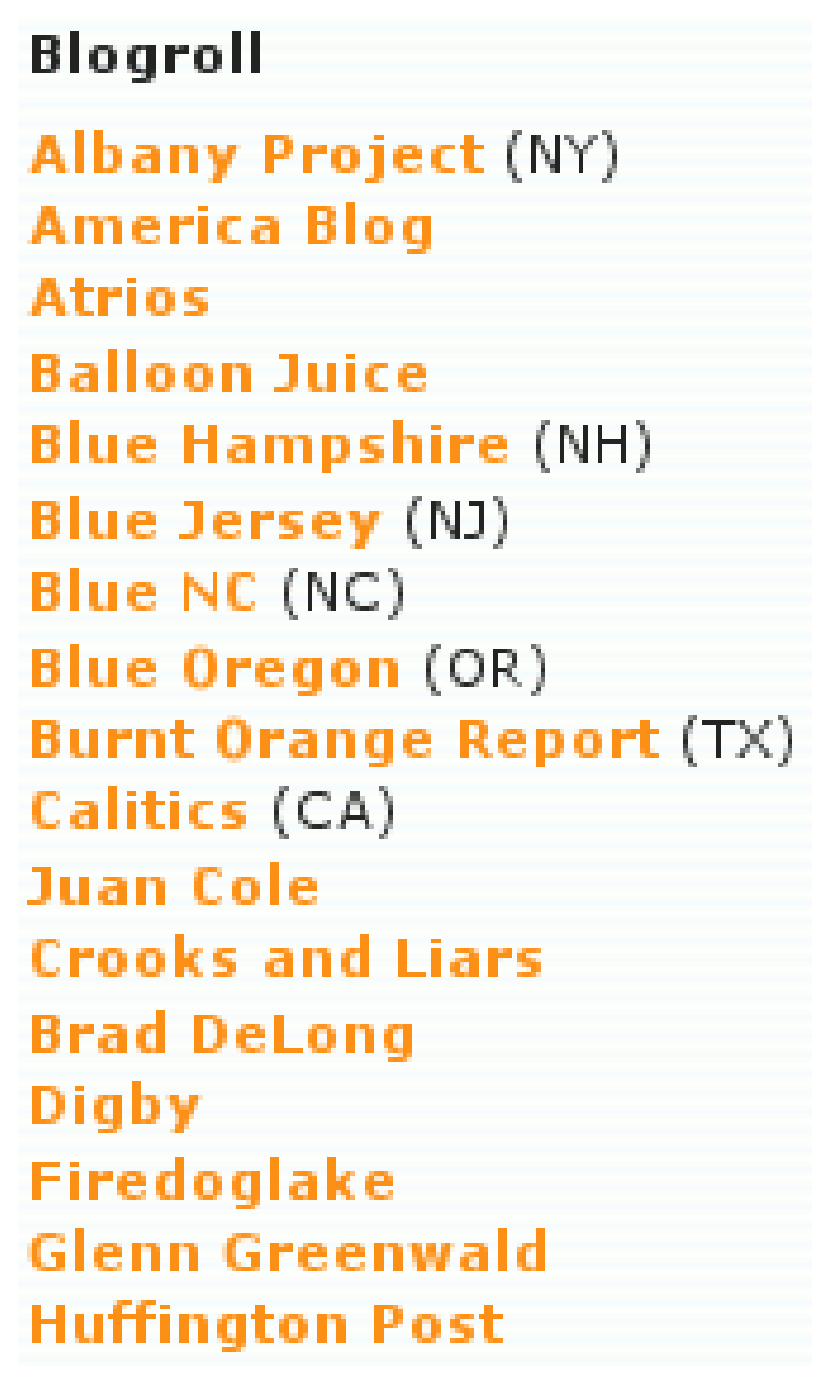
\includegraphics[width=0.9\marginparwidth]{scrsh_dailykos_blogroll}
}

As \citet[\p{806}]{dieberger97} argues the Web's growth, even at it's modest
size of 1997 compared to it's staggering size over 10 years later, have
implications on how easily it is to locate information. By creating pointer
pages, and now socially shared bookmarking services, users are imposing a
structure on the web. By navigating these kinds of interlinked hyperlink
collections it could be that users are getting access to more related and
higher quality information. Sharing a hyperlink, either on you web page or
trough a bookmarking service, requires a conscious effort. One would believe
that people only choose to do so for information they find interesting.

\subsubsection{Item Annotation}

In addition to being a modern form of pointer pages, social bookmarking
with del.icio.us introduced a new way to annotate all kinds of
items (photos, articles, wine, books, videos, music, and so on).
By applying textual key words to
bookmarks\dash{}and later other types of content\dash{}users were able to
browse such collections in new ways. These key words have been popularized as
\term{tags} and the act of applying them is called \term{tagging}%
\sidenote{
  Tagging was discovered by Joshua Schachter when he kept a plain text file
  with a list of all his web page bookmarks. He annotated these bookmarks by
  introducing single-worded labels prefixed with a number sign (\#). He could
  then easily search his bookmarks file with these labels by prefixing
  searches with the number sign. Schachter later introduced tagging to the
  masses by creating the del.icio.us social bookmarking site
  \citep[\p{92}]{weinberger07}.
}.
Joshua Schachter, the creator of del.icio.us, highlight tagging as it's most
essential feature\dash{}the feature that set it apart from the competition
\cite[\p{225}]{livingston07}. Tagging solves a recurring problem with
using traditional folder or hierarchical categorization of items like
bookmarks. In such a system an item can only go in one folder. With
tags items can live in several categories at once
\citep[\p{93}]{weinberger07}.

Tagging enables a user driven taxonomy (classification)
which is often called an \term{folksonomy}\dash{}a combination of the words
\emph{folk} and \emph{taxonomy}. A folksonomy is a strictly bottom-up
approach because of the lack of any predefined taxonomic structure. They
therefore rely on \postquote[\p{31}]{marlow06}{%
  shared and emergent social structures and behaviors, as well as related and
  linguistic structures of the user community}
Since we're mainly interested in the navigational possibilities tagging can
give us we're leaving out a deeper discussion of the benefits and drawbacks
of folksonomies. \citet{golder06} and \citet{marlow06} gives a detailed
account of the tag usage and structure in respectively del.icio.us and
\project{Flickr}%
\sidenote{%
  Flickr is a social image sharing web site available at
  \url{http://flickr.com}. We dig deeper into Flickr when
  we analyze it's social navigation capabilities in
  \sectionref{analysis.flickr}.
}.

As we've described tagging is often a collaborative process. Some web pages
for instance give suggestions for tags if the item you're annotating have
been tagged by others previously. Based on our own usage of collaborative
tagging system we seem to be more inclined to use some or all of these tags
than to come up with their own. In other words our vocabulary is influenced
by the user community. \citet[\p{186}]{sen06} confirmed our personal
observations when they found that the community influence affects the
vocabulary of tags an individual uses. \citet[\p{355}]{farooq07} conducted
similar studies on a collaborative tagging service where the user interface
did not display the tags other people had applied for a similar resource.
They did not find any significant reuse of tags from other users and explained
this discrepancy with the lack of visualization of other user's tags as
evident in other bookmarking services. This means that one can influence
the tag vocabulary of users when they are applying tags by showing other
user's vocabulary usage.

In addition to being shown other people's tags when tagging one can also
be given a list of the tags oneself have previously used.
Under such circumstances \citet[\p{185}]{sen06} found that the probability
of using a previously used tag rose as the amount of tags the user had
applied increased. \citet[\p{355}]{farooq07} validated this phenomena
by showing similar results from another collaborative tagging system.

Applying your own tags for a given resource makes sense if you're annotating a
bookmark. You have your own representation of the bookmark given by the name
you gave it and the tags you chose to apply. Since a bookmark is distinguished
by a \abbr{URL} others can have other representations of the same resource.
For other content items as photos in a photo sharing site it may make more
sense to allow every user, not only the creator, to apply globally visible
tags for this single item. There is then only one representation of this item
and it's tags.
Tags need not be collaboratively created. When one for instance are tagging
one's personal email messages it makes sense to keep such behavior private.

As we've seen folksonomies can be separated by their level of tag sharing
(private systems, fully open systems, and systems with user control over
what gets shared) and tag scope (are tags applied to an item globally
or do they belong to separate users).
\citet[\pp{34}{36}]{marlow06} gives a very detailed account of how tagging
systems can differ in design and how such variations can result in
folksonomies with different characteristics.

Annotating items seems to have benefits with regards to describing the items
and use them for categorization. But how does this relate to navigation?
By giving users a means to better describe various items it will hopefully be
easier for others to use this information in navigation\dash{}they will
hopefully easier find the items or resources they are searching.

The seemingly most used way to display tags for navigation is by generating
a so called \term{tag cloud}%
\sidenote{
  According to \citet{wikipedia08tagcloud} the first usage of tag clouds
  was on Flickr for showing tags applied to photos. The idea of such
  visualization seem to have come from \citet{flanagan03}'s display
  of search terms used when accessing his web site.
}.
\prequote[\p{1}]{fokker06}{%
  succinctly defines the technique as}{%
    The cloud is a representation of the frequency-based relation of tags}
This means that a tag cloud is used to visualize how frequent various tags
are applied to one or more objects. Frequenzy is usually portrayed by varying
the font size based on usage. A highly utilized tag has a large font size
while less used tags have smaller font sizes. There are usually several levels
of font sizes in a tag cloud to visualize how popular tags are in relation to
others. Sometimes colors is used in addition to font size to even better
distinguish amongst the frequenzy of tag usage by showing the most used tags
with a higher contrast color than less used tags. Lastly tags are listed
alphabetically giving a visualization that in many ways resembles clouds of
various sizes in the sky.
\figureref{scrsh.flickr.tagcloud} shows an example of a tag cloud
for photos on Flickr.

Tag clouds are socially constructed tools for navigation. 
% more here

\citet{jarrett05} gives an account into how they created a syndication
aggregator with tagging support. They designed their application with a focus
on enabling users to easily find relevant syndication items trough
social navigation. The cornerstone of their approach to social navigation was
enabling a folksonomy the users could navigate for finding syndication
items. Sadly user studies and evaluations
of the merits of this approach to social navigation is non-existent.

\citet{millen06} on also gives an account of how they used collaborative
tagging with a focus on enabling social navigation in their
\project{Dogear} social bookmarking system. Fortunately they have conducted
studies on the merits of such an approach to social navigation. When users
were navigating bookmarks they most frequently browsed bookmarks for a given
user. But browsing by a tag was not much less frequent, supporting evidence of
the usefulness of folksonomies for enabling social navigation. In addition
it was found that of all bookmarks clicked, 74\% was of other user's
bookmarks, a degree the authors interpret as evidence of a high degree of
social navigation within the social bookmarking system.

\citet[\p{1}]{fokker06} argues that collaborative tagging is ideal
when you have objects where one can not easily perform keyword search on the
information it contains. If these objects are composed of video content tags
can serve as an augmenter for performing keyword based searches as one could
do in textual content. They leveraged tagging in this manner when creating a
prototype of Wikipedia supporting video content\dash{}using tags as the
principle navigation mechanism. By doing so \citet[\p{2}]{fokker06}
saw the need for bootstrapping the availability of tags so that users would be
more inclined to create their own tags. Their solution was to algorithmically
create tags based on the contents of Wikipedia and hoped the existence of
these tags would stimulate users to start tagging themselves.

Tagging have it's shortcomings. Tags could be misspelled, tags with the same
name are not always  homonymous, and tags with the same meaning does not
always have the same name because of synonyms \citep[\p{59}]{aurnhammer06}. In
addition \citet[\p{943}]{li07} argues that browsing tags by traditional
methods with keyword search or tag clouds is inefficient when the set of tags
are quite large. They implemented a system to mediate the synonymy and
homonymy problems with tags in addition the the problems with browsing a large
collection of tags. Their solution to tag ambiguity
was to generate the semantic concept%
\sidenote{
  Generating the semantic concept of a tag means to derive it's meaning in
  a broader sense. Say for instance that a user is browsing for
  \emph{movies}. An algorithm that generates the semantic meaning of
  \emph{movies} could for instance map this to the concept of \emph{movie},
  where such tags as \emph{movies}, \emph{film}, and \emph{flick} could be
  associated with the concept of \emph{movie}.
}
of a tag and use that semantic meaning
when the user is looking for resources through tag browsing
\citep[\p{946}]{li07}.
As \citet[\p{95}]{weinberger07} argues this problem
with tag ambiguity does not really matter when the collection of annotated
items becomes sufficiently large. One would only be concerned with such
matters if one need to find every possible item that is associated with a
concept.
\citet[\p{5}]{hassan06} applied the notion of the semantics of tags to
generate what they concider to be a better solution for displaying tag clouds.
Similar tags based on semantics are grouped together horizontally in what they
call clusters. These clusters is then again sorted vertically based on their
semantic relation.

The problem of browsing large scale tagging collections is tackled by
inferring a hierarchy%
\sidenote{
  Once can tag object by several levels of abstraction. One can for instance
  tag a movie with \emph{movie} to identify what it is. Then one could use
  the tags \emph{comedy}, \emph{romanticcomdey}, and \emph{norwegian} for
  describing the object's features. One could computationally derive an
  hierarchy from the varying levels of abstraction in such tags saying
  that \emph{comedy} is the child of \emph{movie} and \emph{romanticcomedy}
  is the child of \emph{comedy}.
}
from the flat tag space \citep[\pp{946}{948}]{li07}.

We've seen that item annotation or tagging can be used to annotate items for
describing the information they convey and
thereby afford navigation. As we'll see in
\sectionref{background.social.navigation.applied.forms.recommendations}
annotations can also be used for describing the quality, importance, or
usefulness of an item and thereby potentially creating recommendations.

\subsubsection{Interaction History Trails}
\label{section:background.social.navigation.applied.forms.interaction.history}
% in the wild: trail-fire, new hoodwink.d like Greasemonkey service
% history-rich objects: hill92, hill94

In a classic article \citet{wexelblat99} contrasts the digital world of
computers with our physical world with respect to the formers lack of history.
In our traditional world we exploit such historical information traces
\postquote[\p{270}]{wexelblat99}{%
  to guide our actions, to make choices, and to find things of
  importance or interest}
It's argued that this apparent lack of history in computerized systems must
be sorted out such that future users can take advantage
of past users' historical traces left when they were working
on solving problems similar to the current user's.
A possible remedy for this problem on the Web is put forth in the authors'
\project{Footprints} system\dash{}an navigational aid as an extension to
normal web browsers, visualizing interaction history of past users enabling
current users to navigate this history.

This interaction history consists of several navigation trails which are
\postquote[\p{273}]{wexelblat99}{%
  coherent sequences of nodes followed by an individual}
The idea of such trails of navigation far preceded \citeauthor{wexelblat99}
as they were envisioned by \citet{bush45} when he proposed the infamous
theoretical computer-like system named the \project{Memex}%
\sidenote[-15\onelineskip]{
  The Memex was not envisioned as a computer system but as an
  mechanical system consisting of a set of controls hooked up
  to a microfilm reader and camera. It was
  theorized by \citeauthor{bush45} to be a system for handling
  a persons entire collection of documents, books, and communication.
  It was
  important that a user would be able to access this information with great
  speed and flexibility. An integral part of enabling such efficient access
  was a user' and content providers' ability to introduce trails between
  information items. \citeauthor{bush45}'s writing about trails
  inspired hypertext \citep[\p{86}]{nelson65} which in turn was the grand idea
  behind the World Wide Web \citep[\p{49}]{myers98}.
}.
\citeauthor{bush45} describes a scenario where users are building trails
explicitly, inserts comments if needed, and gives it a name.
\citeauthor{wexelblat99} on the other hand
implemented a system where trails are automatically collected using a set of
heuristics to identify browsing behavior representing a coherent navigation
trail.
\citeauthor{bush45} wrote his essay before the invention of computer networks
and he thinks of each Memex as a separate island. Sharing of trails is
possible trough an exportation and following importation process, making it an
explicit action for it's users.
The Footprints system makes the social process of sharing trails implicit and
transparent to it's users\dash{}multiplayer is forced.

Controlled user studies by \citeauthor{wexelblat99} did partially falsify
their pre-test hypothesis of Footprint's ability to let users find more
relevant results during a specific browsing task and that this browsing
would be more efficient. The group using the history-enriched system reported
significant lower values of mean page count in their browsing task. No
significantly difference in results returned was found between users of a
plain web browser and users with a browser enhanced with Footprints. They also
found that people experienced in the problem domain of the browsing task were
to a larger degree able to take advantage of interaction history than novices.
\citeauthor{wexelblat99} attributed this to experienced people's ability to
have a clearer mental model of the information one was browsing.

% Juggler discourse here, maybe

\subsubsection{Populated Space}

A \term{populated space} is
\postquote[\p{41}]{dieberger00b}{%
  an information space in which other people can be encountered}
By providing online awareness users can see where other users are moving and
spending time. In contrast to interaction history where such behavior is
stored for later retrieval a populated space only shows what others are doing
in real-time.

\project{Kalas} \citep{svensson05}, a system for interacting with food
recipes, uses the idea of populated space to enable user awareness. Kalas is
also a recommendation system and is in our opinion one of the best studied
social navigation systems. We'll therefore come back to
\citeauthor{svensson05}'s evaluations of different social
navigation techniques.

\subsubsection{Collaborative Filtering}
\label{section:background.social.navigation.applied.forms.collaborative.filtering}
% introduce earlier cited goldberg92 article and more recent work.
% collaborative filtering is often used for recommendation systems
% look at the benefits of implicit feedback in contrast to explicit feedback
% with regard to recommendation systems as highlighted by claypool01.

\todo{Discuss the most important articles and implementations.}

\subsubsection{Recommendations}
\label{section:background.social.navigation.applied.forms.recommendations}

So called \term{recommender systems} are often based on collaborative
filtering principles. % continue discussion and citing.

One of the two forms of social navigation found in
\project{Knowledge Sea}\dash{}a digital educational
library\dash{}is recommendations by item
annotation \citep[\p{13}]{brusilovsky05}. Users can leave their emphatic marks
on content and thereby specify it's usefulness. Questionnaires showed that a
fair majority of users was agreeable to the use of such recommendations
\citeyearpar[\p{15}]{brusilovsky05} and log analysis strengthened
the impression
\begin{fullquote}[\p{38}]{brusilovsky05}{had by showing that}
  Social navigation support and specifically
  annotation-based social navigation increases the chance of
  accessing a resource dramatically.
\end{fullquote}

Advanced algorithms known in the field of collaborative filtering
and recommendation systems have been used together with folksonomies
consisting of collaborative tags
\citep[\pp{112}{113}]{wu06}. Preliminary studies have shown positive
results when harnessing such social knowledge with filtering algorithms
as opposed to traditional folksonomy representation
\citep[\p{114}]{wu06}. Such a folksonomy could hoverer interfere with an
existing recommendation system. \citet[\p{190}]{sen06} found that the
introduction of tagging and tag display in their established
movie recommendation system interfered with some of the users primary
objective: finding interesting movies. Note that this dislike of a
folksonomy was more likely to be present for users familiar with the old
movie recommendation system sans any folksonomy. New users having not
witnessed the recommendation system without any folksonomy seemed more
acceptant towards tagging.

\subsubsection{Social Texture}
% activity, usage, edit/read wear
% footprints users edit/read wear for instance.

\begin{figure}
  \captionstyle{\raggedright}
  \begin{whole}
    \begin{minipage}[t]{0.475\wholewidth}
      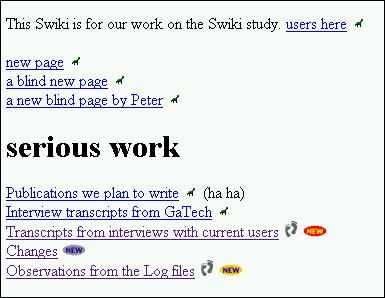
\includegraphics[width=\textwidth]{scrsh_coweb_contextual}
      \caption[CoWeb Contextual Cues]{%
        CoWeb Contextual Cues,
        retrieved January 25, 2008, from
        \url{http://homepage.mac.com/juggle5/WORK/publications/SwikiWriteup.html}.
      }
      \label{figure:scrsh.coweb.contextual}
    \end{minipage}
    \hfill
    \begin{minipage}[t]{0.475\wholewidth}
      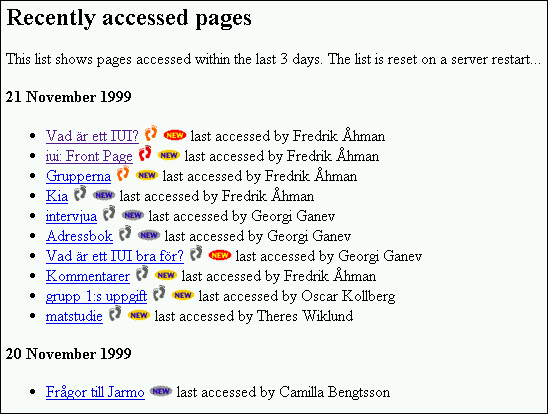
\includegraphics[width=\textwidth]{scrsh_coweb_global}
      \caption[CoWeb Global Cues]{%
        CoWeb Global Cues,
        retrieved January 25, 2008, from
        \url{http://homepage.mac.com/juggle5/WORK/publications/SwikiWriteup.html}.
      }
      \label{figure:scrsh.coweb.global}
    \end{minipage}
  \end{whole}
  \normalcaption
\end{figure}

We use \term{social texture} to describe socially constructed annotations or
visualizations which may be used for navigation or in some form guide
users in navigational choices.

Social texture ties in with the forms of social navigation we've
recently discussed. Tagging for instance is a social texture.
The interaction history systems we've discussed uses forms of visualizations
in close proximity to hyperlinks to convey their degree of usage. This is also
a form of social texture.

The first forms of social texture used in computer systems to our knowledge is
\citet{hill92}'s usage of \term{computational wear} which is an analogy for
the wear physical objects experience when used. They modify a text editor to
show both wear related to document edits and readings of documents. This wear
is graphically visualized trough the editor's scroll bar.
The concept of edit and read wear has since been used on the Web in for
instance the Footprints system \citep{wexelblat99}.

\citet{dieberger00a} modified \project{CoWeb}\dash{}a collaborative Web space
modelled after Ward Cunningham's famous Wikis\dash{}to include interaction
history visualization hoping to make it a more social space, enabling social
navigation. They visualized other users' access of different pages both by
including a global list of such behavior and contextual cues about access
next to internal hyperlinks.
It was inferred by \citeauthor{dieberger00a} that markers of interaction
history increased the overall activity on the web page during a user study.
They also learned that it's important to both provide both global and
contextual interaction history cues.

\citet{xu06} modified a Wiki in even more elaborate ways
with the aim of integrating several social navigational mechanisms.
They used read-wear information for creating social
texture in the Wiki both in-line pages, on a page level, and on a global
level. \citeauthor{xu06} took the approach of displaying read-wear in real
time, thus making the system a populated space. To make such an approach
useful the Wiki needs a certain amount of users present at all times. If
it's not frequently trafficked it would probably be better to represent
historical read-wear as done in CoWeb \citep[\p{220}]{dieberger00a}. Both
contextual and global use of such social texture can be seen in
\figureref{scrsh.coweb.contextual} and \figureref{scrsh.coweb.global}.

\project{virtPresenter} is a hypermedia based lecture viewer where read-wear
have been used to visualize a groups' interaction with continuous content
\citep{mertens06}. By following the traces other users have left current users
can interpret what's the most sought after parts of a lecture. The
visualization is implemented in ways similar to \citet{hill92} by showing
graphs of usage in line with a timeline selector and can be seen in
\figureref{scrsh.virtpresenter.timeline}.

We discussed KnowledgeSea regarding it's use of recommendations in
\sectionref{background.social.navigation.applied.forms.recommendations}.
The system also incorporates what the authors calls
\term{traffic-based social navigation}
\citep[\p{12}]{brusilovsky05}\dash{}in other words history based
visualizations in the form of read-wear. The access of different articles in
the digital library are recorded and the degree of usage is then visualized in
the form of different color tones where darker indicates a more popular
resource. Such visualization is used consistently throughout the web site. A
questionnaire revealed that in excess of 70\%
\citeyearpar[p.15]{brusilovsky05} of the users
found such history based visualizations useful and appropriate.

\begin{figure}
  \centering
  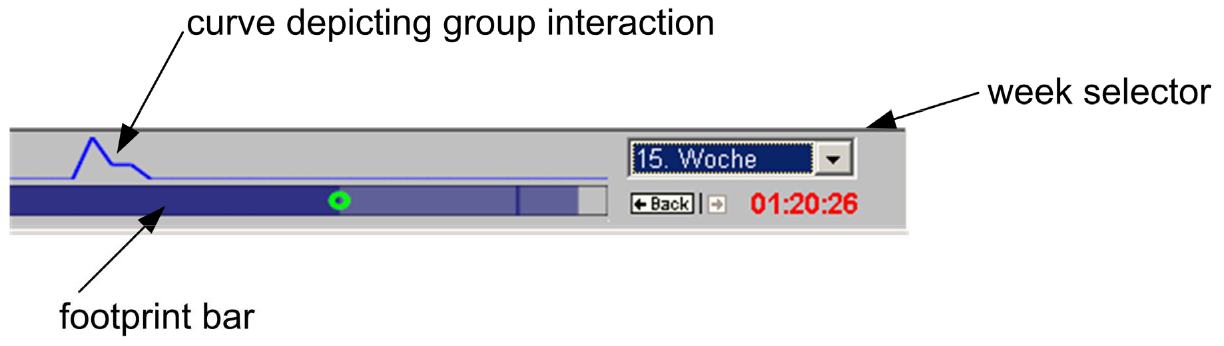
\includegraphics[width=0.9\textwidth]{scrsh_virtpresenter_timeline}
  \caption[virtPresenter Timeline]{
    virtPresenter Timeline \citep[\p{43}]{mertens06}.
  }
  \label{figure:scrsh.virtpresenter.timeline}
\end{figure}


\subsubsection{Search}
% social search articles and semantic web/search article
% not that relevant as we're focusing on navigation trough browsing
% brusilovsky05 have some discussion of using social navigation in search
% results

\subsection{Usefulness}
% dieberger00b:
%   filtering: HEE - find most relevant info
%              RecSys - pick items from a large space
%   quality:   HEE - find quality info (interesting, valid)
%   social affordance: HEE - users aware of each other
%                          - social experience
%                      - space is alive
%                        - not only affect navigation
%                          - stay longer in the space
%                          - relaxed
%                          - try new features

\citet{svensson05} performed a throughout evaluation of the Kalas system and
two issues in perspective of social navigation:

\begin{enumerate}
  \item Will social navigation enable users to navigate more efficiently?
  \item Do social navigation increase the perceived subjective quality of
    a navigation process?
\end{enumerate}

Server logs were statistically mined and more in depth qualitative interviews
were conducted. The results showed that people tended to move to the most
populated part of system and used recommendations for helping select which
items to navigate. \citeauthor{svensson05} also found that the subjects
overall had a positive impression of the social features of the system. They
seemed more interested in expressing themselves trough such features than
using information from others to help their navigation process.

Favorable results for the effectiveness of social navigation was observed
during a simulation experiment conducted by \citeauthor{riedl03}. In most
circumstances social navigation had favorable results in efficiency contrasted
with asocial navigation. It's important to note that social navigation
decreased the effectiveness of navigation in some instances of their
simulations \citeyearpar[\p{365}]{riedl03}.
Interestingly, it was discovered that social navigation was more
beneficial in environments with high uncertainty%
\sidenote[-5\onelineskip]{
  \prequote[\p{363}]{riedl03}{%
    says that the two sources of such uncertainty is}{%
      arising from the correctness of the information gained in any state,
      and the potential difficulty of reaching that state to obtain
      the information}
}
than environments with higher certainty\dash{}provided that the
simulated agents could reach the social media
\citeyearpar[\p{368}]{riedl03}. 

\section{Building on Top of the Web}
\label{section:building.on.top.of.the.web}
% Greasemonkey, hoodwink.d, new hoodwink.d service
% browser extensions related, Greasemonkey itself a extension, but
% thinking about specialized plugins for enabling interaction on top of other
% web pages.
% mashups kind of related, maybe put inside web2.0 part or separate part
% open apis is the fuel for mashups. possible without by screen scraping, but
% not as convenient and safe (upgrades on the pages we're scraping)
% facebook, open social. applications on top of social network sites.
% installed base of users and relationships already in place.

Going in and making changes to an existing web site can be both an
daunting and time consuming task. First one have to establish a trustworthy
relationship with the creators of such a site so that they are certain
you're not introducing bugs in their production software. Secondly, grasping
the code base, third party libraries, and development tools of such a software
project demands a lot of upfront effort before any real development work can
begin. This goes against the prototypical process we intended to use while
experimenting with \urort{}.

Even though we've had an ongoing dialog with the developers of \urort{} we
decided to create our prototype as a layer on top of their site.
By using an
extension
for the leading open source%
\sidenote{
  The \project{Firefox} web browser. Available at \url{http://firefox.com}.
}
web browser we were able to create a script which
made changes and additions to the way \urort{}
were presented to users who were participating in our study.
Such an approach would hopefully result in a transparent experience for our
end users as long as they have taken the necessary steps to set up the browser
extension and our script.

The idea of creating additional features for a web site in these manners
came from the author's involvement in an underground community based around
the Ruby%
\sidenote{
  Can be retrieved from \url{http://ruby-lang.org}.
}
programming language. \project{Hoodwink.d}%
\sidenote{
  Hoodwink.d's starting point for new users can be seen
  at \url{http://hoodwinkd.hobix.com}.
},
as it's called, is a service that lets members post comments on all kinds of
web sites. These comments are then only visible to the members of the
community.
Hoodwink.d is underground in the sense that it's quite hard to get in to
the community. It's members rarely talk about Hoodwink.d publicly, baring
similarities to the underground fight club in a novel by \citet{palahniuk96}
aptly named \work{Fight Club}%
\oddsidenote[-4\onelineskip]{
  The first two rules of this underground club in the novel of
  \citet[\pp{48}{50}]{palahniuk96}
  clearly describes the attitude members have to outsiders:
  \begin{inparaenum}[(i)]
    \item You don't talk about fight club.
    \item You don't talk about fight club.
  \end{inparaenum}
}.
The home page of Hoodwink.d mimics the community's dedication to secrecy
by obfuscating it's information as can be seen in
\figureref{scrsh.hoodwinkd.obfuscation}.
When the information on the page is viewed without obfuscation%
\oddsidenote{
  The obfuscation can be removed either by turning off \abbr{CSS} support
  in your browser or viewing the page's source.
}
one have to be pretty technical savvy to decipher what the information 
actually means. Simply put users have to change their hosts file
so that it points to two imaginary domain names. Doing so they can point their
browser to these domains and download a script (such scripts are discussed in
\sectionref{selection.stack.client.platform})
that enables the functionality
of Hoodwink.d.%
\oddsidenote{
  Oh no, we just broke the first and second rule of \work{Fight Club}!
}
This approach creates a barrier to entry which only allows the most
technically inclined to enter the community\dash{}allowing for a
high level of technicality in the community's internal discussions
and thereby filtering out so called \term{newbies}
(newcomers and beginners).

\begin{figure}
  \centering
  
\includegraphics[width=0.9\textwidth]{scrsh_hoodwinkd_obfuscation}
  \caption[Hoodwink.d Obfuscation]{
    Obfuscation of Hoodwink.d's home page,
    retrieved March 6, 2008, from
    \url{http://hoodwinkd.hobix.com}.
  }
  \label{figure:scrsh.hoodwinkd.obfuscation}
\end{figure}

\begin{figure}
  \begin{whole}
    \centering
    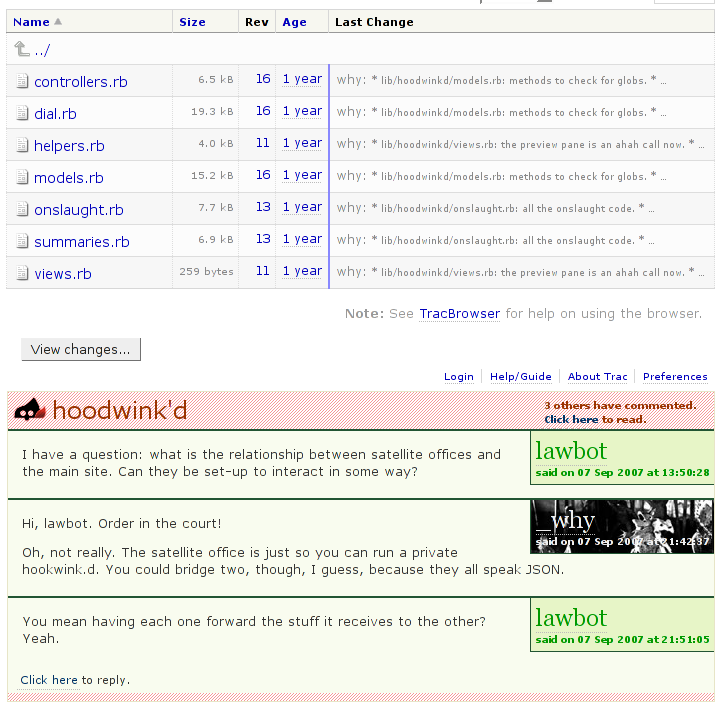
\includegraphics[width=0.9\wholewidth]{scrsh_hoodwinkd_comment_source}
    \caption[Hoodwink.d Comments]{
      Comments on the repository browser of Hoodwink.d's source code,
      retrieved March 7, 2008, from
      \url{http://code.whytheluckystiff.net/hoodwinkd}.
    }
    \label{figure:scrsh.hoodwinkd.comment.source}
  \end{whole}
\end{figure}

Now we finally get to the really interesting part of Hoodwink.d: the features
it enables on top of the Web. One can create a comment visible only to the
community's members on any web page that is supported. This support is not
dependant on the creator of the web site, but the users of Hoodwink.d needs to
record some information of the web site (where the comments should be placed)
to make it supported. \figureref{scrsh.hoodwinkd.comment.source} shows an
example of how these comments are displayed on the repository browser for
the Hoodwink.d source code itself. This page does not natively support
comments. Using Hoodink.d for such means is a very cheap (time wise) option
compared to implementing such features in the repository browser.
They are perceived as being part of the web page itself, even though they
are inserted right after the page is fully loaded.

To tie together these comments a central portal lists
the most recently placed comments (as can be seen in
\figureref{scrsh.hoodwinkd.onslaught.recent}), the most actively commented web
sites, the most recently new supported sites, and the most active users.

\sidefigure{Hoodwink.d Recent Comments}{%
  Recent comments on Hoodwink.d,
  retrieved March 7, 2008, from
  \url{http://hoodwink.d/onslaught}.
  \label{figure:scrsh.hoodwinkd.onslaught.recent}
}{%
  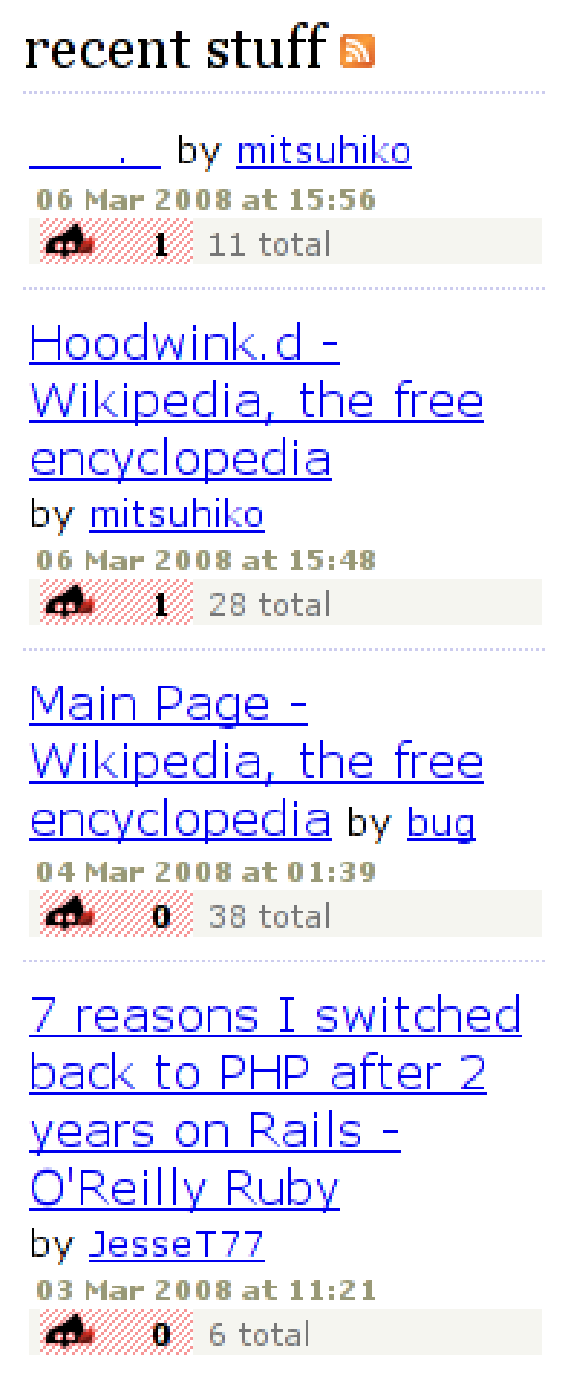
\includegraphics[width=0.9\marginparwidth]{scrsh_hoodwinkd_onslaught_recent}
}
